\documentclass[a4paper, 12pt]{scrartcl}
\usepackage[top=2.5cm, bottom=2.5cm, left=2.5cm, right=2.5cm]{geometry}
\usepackage{mathptmx}
\usepackage{graphicx}
\usepackage{amsmath}
\usepackage{tikz}
\usepackage{pgfplots}
\usepackage{caption}
\usepackage[labelformat=simple]{subcaption}
\usepackage{wasysym}
\usepackage{enumitem}
\renewcommand\thesubfigure{(\alph{subfigure})}
% Strange fisita formatting
\setkomafont{title}{\normalfont\bfseries}
\addtokomafont{disposition}{\rmfamily}
\setkomafont{section}{\large\bfseries}
\setkomafont{subsection}{}
\setkomafont{subsubsection}{\large\bfseries}

\setlist[description]{  font={\bfseries\rmfamily}
}


% Begin the LaTeX document
\begin{document}

% Paper Title
\title{\large \uppercase{Analysis of Big Data Streams to obtain Braking Reliability Information for Train Protection systems}}

% Authors List
\author{\normalsize	
	Pfaff, Raphael*, Elsen, Ingo, Schmidt, Bernd \\ \normalsize	
	FH Aachen University of Applied Sciences, Aachen, Germany \\
	\normalsize \{pfaff, elsen, b.schmidt\}@fh-aachen.de}
\date{}
% Author Affiliations
% Create the title
\maketitle

% Abstract

KEYWORDS - ETCS, braking curve, big data, performance prediction, condition monitoring

ABSTRACT 

Due to the long braking distance of railway systems and the high velocities achieved, railway operation needs to rely on train control systems. At the foundation of these systems are models to predict the motion of the trains, including their anticipated braking curve. Depending on the infrastructure manager, these braking curves need to be achieved with a given safety, which is typically in the rare event region of probabilities.

In current settings, it is typical to develop these so called braking curves either by physical modelling of the train followed by a Monte Carlo simulation or following a heuristic approach, mostly based on the high level of safety over the past centuries.

However, higher developed train protection and control systems, such as the European Rail Traffic Management System (ERTMS) or the Russian KLUB-U System together with current efforts towards quantitative risk analysis, e.g. the European Common Safety Methods, require a more formal approach to communicate the braking curve of a train between rolling stock and infrastructure.

An a priori determined set of braking curves is feasible for trains running in fixed or a limited number of formations, such as multiple unit trains, however in the freight railway system due to its vast amount of different vehicles and possible train setups, the determination of the braking curves is prohibitive.


\section{\uppercase{Introduction}}
\subsection{\uppercase{Railway System Operation (Bernd)}}
%BM235
Among the key differences between road and rail traffic relevant to this work are the composition of trains and wheel-rail contact between steel contact partners. While the latter contributes largely to the energy efficiency of the railways by reducing flexing work of tyres or wheels, it provides only limited tangential force transfer between wheel and rail, resulting in longer braking distances. 

The formation of trains is also an advantage of the railway system, as it reduces labour cost, infrastructure usage and energy consumption of the trains. Depending on infrastructure constraints, train consists of up to 6000 m length are formed. The case under consideration assumes a European setting, limiting the maximum train length in most parts of the network to 740 m \cite{tsiinf}.

The operation of trains, similar to road transport, needs to maintain safe distances between trains on a track to ensure braking before collision with another train or exceeding a so called danger point, e.g. a switch not properly set for the train. Since braked masses are high and adhesion is low compared to road transport, these distances are long and typically require technical safety measures, such as signals.

In Figure \ref{fig:DistanceKeeping}, the different approaches to maintaining train distances are illustrated. In this figure, $s_{b,i}$, $i = 1,2$, denotes the braking distance of train $i$, $t_{l, i}$ the train length and $S$ is a safety margin train. Approach \subref{fig:AbsSpacDist} is the one frequently chosen due to its relative simplicity in implementation. It is however a rather inefficient approach in terms of infrastructure utilisation, with its performance being limited by the block length $l_{bl}$. 

The more performant approach \subref{fig:AbsBakDist} is technologically more demanding since it requires exact and safe position information of the the trains as well as a vehicle side ensurance of train integrity. In this approach, the following train is maintained in a distance that allows it to stop behind the current end of the leading train. This approach is rarely applied in mainline operation, but helps in many mass transit applications to increase network capacity \cite{pachl2011systemtechnik}. 

Approach \subref{fig:RelBakDist} is the most performant of the presented approaches and it resembles normal road transportation. In this scenario, trains are operated such that the following train can stop behind the leading train assuming its deceleration by braking. As can be assumed from the similarity to road transportation, rear-end collisions are prone to be more likely when operating in relative braking distances.
 
\begin{figure}
\begin{center}
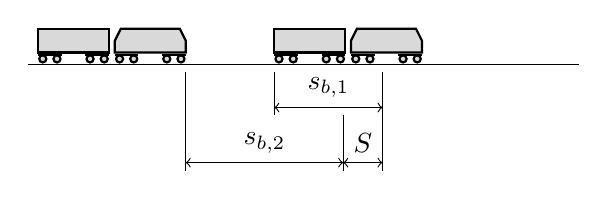
\begin{tikzpicture}
% Top of rail
\draw[] (-2, -.15) -- (5, -.15);
% Distances
\draw[] (0, -.25) -- (0, -1.5);
\draw[] (2.5, -.25) -- (2.5, -1.5);
\draw[] (1.125, -.25) -- (1.125, -.8);
\draw[] (2, -.8) -- (2, -1.5);
\draw[<->] (1.125, -.7) -- (2.5,-.7) node[pos = 0.5, above] {$s_{b,1}$};
\draw[<->] (0, -1.4) -- (2,-1.4) node[pos = 0.5, above] {$s_{b,2}$};
\draw[<->] (2, -1.4) -- (2.5,-1.4) node[pos = 0.5, above] {$S$};
\begin{scope}[scale = 0.15]
	%Loco 1
\begin{scope} [shift = {(-6,0)}]
\draw[thick, fill = gray!30] (0,0) -- (0,1) -- (.5,2) -- (5.5,2) -- (6,1) -- (6,0) -- cycle;
\draw[thick] (0, -.2) -- (2, -.2); 
\draw[thick, fill = gray!30] (.4, -.55) circle (.3);
\draw[thick, fill = gray!30] (1.6, -.55) circle (.3);
\begin{scope} [shift = {(4,0)}]
\draw[thick] (0, -.2) -- (2, -.2); 
\draw[thick, fill = gray!30] (.4, -.55) circle (.3);
\draw[thick, fill = gray!30] (1.6, -.55) circle (.3);
\end{scope}
\end{scope}
%Wagon 1
\begin{scope} [shift = {(-12.5,0)}]
\draw[thick, fill = gray!30] (0,0)  -- (0,2) -- (6,2) -- (6,0) -- cycle;
\draw[thick] (0, -.2) -- (2, -.2); 
\draw[thick, fill = gray!30] (.4, -.55) circle (.3);
\draw[thick, fill = gray!30] (1.6, -.55) circle (.3);
\begin{scope} [shift = {(4,0)}]
\draw[thick] (0, -.2) -- (2, -.2); 
\draw[thick, fill = gray!30] (.4, -.55) circle (.3);
\draw[thick, fill = gray!30] (1.6, -.55) circle (.3);
\end{scope}
\end{scope}

\end{scope}
\begin{scope} [shift = {(3,0)}, scale = 0.15]
	%Loco 1
\begin{scope} [shift = {(-6,0)}]
\draw[thick, fill = gray!30] (0,0) -- (0,1) -- (.5,2) -- (5.5,2) -- (6,1) -- (6,0) -- cycle;
\draw[thick] (0, -.2) -- (2, -.2); 
\draw[thick, fill = gray!30] (.4, -.55) circle (.3);
\draw[thick, fill = gray!30] (1.6, -.55) circle (.3);
\begin{scope} [shift = {(4,0)}]
\draw[thick] (0, -.2) -- (2, -.2); 
\draw[thick, fill = gray!30] (.4, -.55) circle (.3);
\draw[thick, fill = gray!30] (1.6, -.55) circle (.3);
\end{scope}
\end{scope}
%Wagon 1
\begin{scope} [shift = {(-12.5,0)}]
\draw[thick, fill = gray!30] (0,0)  -- (0,2) -- (6,2) -- (6,0) -- cycle;
\draw[thick] (0, -.2) -- (2, -.2); 
\draw[thick, fill = gray!30] (.4, -.55) circle (.3);
\draw[thick, fill = gray!30] (1.6, -.55) circle (.3);
\begin{scope} [shift = {(4,0)}]
\draw[thick] (0, -.2) -- (2, -.2); 
\draw[thick, fill = gray!30] (.4, -.55) circle (.3);
\draw[thick, fill = gray!30] (1.6, -.55) circle (.3);
\end{scope}
\end{scope}

\end{scope}
\end{tikzpicture}
\subcaption{Operation in relative braking distance}
\label{fig:RelBakDist}
\end{center}
\begin{center}
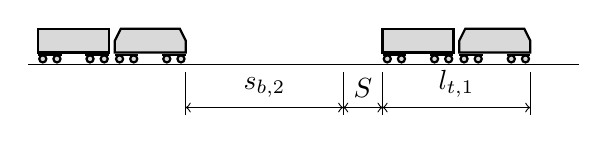
\begin{tikzpicture}
% Top of rail
\draw[] (-2, -.15) -- (5, -.15);
% Distances
\draw[] (0, -.25) -- (0, -.8);
\draw[] (2, -.25) -- (2, -.8);
\draw[] (4.375, -.25) -- (4.375, -.8);
\draw[] (2.5, -.25) -- (2.5, -.8);
\draw[<->] (2.5, -.7) -- (4.375,-.7) node[pos = 0.5, above] {$l_{t,1}$};
\draw[<->] (0, -.7) -- (2,-.7) node[pos = 0.5, above] {$s_{b,2}$};
\draw[<->] (2, -.7) -- (2.5,-.7) node[pos = 0.5, above] {$S$};
\begin{scope}[scale = 0.15]
	%Loco 1
\begin{scope} [shift = {(-6,0)}]
\draw[thick, fill = gray!30] (0,0) -- (0,1) -- (.5,2) -- (5.5,2) -- (6,1) -- (6,0) -- cycle;
\draw[thick] (0, -.2) -- (2, -.2); 
\draw[thick, fill = gray!30] (.4, -.55) circle (.3);
\draw[thick, fill = gray!30] (1.6, -.55) circle (.3);
\begin{scope} [shift = {(4,0)}]
\draw[thick] (0, -.2) -- (2, -.2); 
\draw[thick, fill = gray!30] (.4, -.55) circle (.3);
\draw[thick, fill = gray!30] (1.6, -.55) circle (.3);
\end{scope}
\end{scope}
%Wagon 1
\begin{scope} [shift = {(-12.5,0)}]
\draw[thick, fill = gray!30] (0,0)  -- (0,2) -- (6,2) -- (6,0) -- cycle;
\draw[thick] (0, -.2) -- (2, -.2); 
\draw[thick, fill = gray!30] (.4, -.55) circle (.3);
\draw[thick, fill = gray!30] (1.6, -.55) circle (.3);
\begin{scope} [shift = {(4,0)}]
\draw[thick] (0, -.2) -- (2, -.2); 
\draw[thick, fill = gray!30] (.4, -.55) circle (.3);
\draw[thick, fill = gray!30] (1.6, -.55) circle (.3);
\end{scope}
\end{scope}

\end{scope}
\begin{scope} [shift = {(4.375,0)}, scale = 0.15]
	%Loco 1
\begin{scope} [shift = {(-6,0)}]
\draw[thick, fill = gray!30] (0,0) -- (0,1) -- (.5,2) -- (5.5,2) -- (6,1) -- (6,0) -- cycle;
\draw[thick] (0, -.2) -- (2, -.2); 
\draw[thick, fill = gray!30] (.4, -.55) circle (.3);
\draw[thick, fill = gray!30] (1.6, -.55) circle (.3);
\begin{scope} [shift = {(4,0)}]
\draw[thick] (0, -.2) -- (2, -.2); 
\draw[thick, fill = gray!30] (.4, -.55) circle (.3);
\draw[thick, fill = gray!30] (1.6, -.55) circle (.3);
\end{scope}
\end{scope}
%Wagon 1
\begin{scope} [shift = {(-12.5,0)}]
\draw[thick, fill = gray!30] (0,0)  -- (0,2) -- (6,2) -- (6,0) -- cycle;
\draw[thick] (0, -.2) -- (2, -.2); 
\draw[thick, fill = gray!30] (.4, -.55) circle (.3);
\draw[thick, fill = gray!30] (1.6, -.55) circle (.3);
\begin{scope} [shift = {(4,0)}]
\draw[thick] (0, -.2) -- (2, -.2); 
\draw[thick, fill = gray!30] (.4, -.55) circle (.3);
\draw[thick, fill = gray!30] (1.6, -.55) circle (.3);
\end{scope}
\end{scope}

\end{scope}
\end{tikzpicture}
\subcaption{Operation in absolute braking distance}
\label{fig:AbsBakDist}
\end{center}
\begin{center}
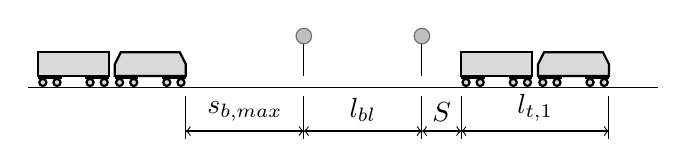
\begin{tikzpicture}
% Top of rail
\draw[] (-2, -.15) -- (6, -.15);
% Distances
\draw[] (0, -.25) -- (0, -.8);
\draw[] (1.5, -.25) -- (1.5, -.8);
\draw[] (3, -.25) -- (3, -.8);
\draw[] (5.375, -.25) -- (5.375, -.8);
\draw[] (3.5, -.25) -- (3.5, -.8);
\draw[<->] (3.5, -.7) -- (5.375,-.7) node[pos = 0.5, above] {$l_{t,1}$};
\draw[<->] (0, -.7) -- (1.5,-.7) node[pos = 0.5, above] {$s_{b,max}$};
\draw[<->] (3, -.7) -- (3.5,-.7) node[pos = 0.5, above] {$S$};
\draw[<->] (1.5, -.7) -- (3,-.7) node[pos = 0.5, above] {$l_{bl}$};
%Signals
\draw (1.5, 0) -- (1.5, .4) node[circle, draw, fill = gray, opacity = .5, above, inner sep = 2pt] {};
\draw (3, 0) -- (3, .4) node[circle, draw, fill = gray, opacity = .5, above, inner sep = 2pt] {};
\begin{scope}[scale = 0.15]
	%Loco 1
\begin{scope} [shift = {(-6,0)}]
\draw[thick, fill = gray!30] (0,0) -- (0,1) -- (.5,2) -- (5.5,2) -- (6,1) -- (6,0) -- cycle;
\draw[thick] (0, -.2) -- (2, -.2); 
\draw[thick, fill = gray!30] (.4, -.55) circle (.3);
\draw[thick, fill = gray!30] (1.6, -.55) circle (.3);
\begin{scope} [shift = {(4,0)}]
\draw[thick] (0, -.2) -- (2, -.2); 
\draw[thick, fill = gray!30] (.4, -.55) circle (.3);
\draw[thick, fill = gray!30] (1.6, -.55) circle (.3);
\end{scope}
\end{scope}
%Wagon 1
\begin{scope} [shift = {(-12.5,0)}]
\draw[thick, fill = gray!30] (0,0)  -- (0,2) -- (6,2) -- (6,0) -- cycle;
\draw[thick] (0, -.2) -- (2, -.2); 
\draw[thick, fill = gray!30] (.4, -.55) circle (.3);
\draw[thick, fill = gray!30] (1.6, -.55) circle (.3);
\begin{scope} [shift = {(4,0)}]
\draw[thick] (0, -.2) -- (2, -.2); 
\draw[thick, fill = gray!30] (.4, -.55) circle (.3);
\draw[thick, fill = gray!30] (1.6, -.55) circle (.3);
\end{scope}
\end{scope}

\end{scope}
\begin{scope} [shift = {(5.375,0)}, scale = 0.15]
	%Loco 1
\begin{scope} [shift = {(-6,0)}]
\draw[thick, fill = gray!30] (0,0) -- (0,1) -- (.5,2) -- (5.5,2) -- (6,1) -- (6,0) -- cycle;
\draw[thick] (0, -.2) -- (2, -.2); 
\draw[thick, fill = gray!30] (.4, -.55) circle (.3);
\draw[thick, fill = gray!30] (1.6, -.55) circle (.3);
\begin{scope} [shift = {(4,0)}]
\draw[thick] (0, -.2) -- (2, -.2); 
\draw[thick, fill = gray!30] (.4, -.55) circle (.3);
\draw[thick, fill = gray!30] (1.6, -.55) circle (.3);
\end{scope}
\end{scope}
%Wagon 1
\begin{scope} [shift = {(-12.5,0)}]
\draw[thick, fill = gray!30] (0,0)  -- (0,2) -- (6,2) -- (6,0) -- cycle;
\draw[thick] (0, -.2) -- (2, -.2); 
\draw[thick, fill = gray!30] (.4, -.55) circle (.3);
\draw[thick, fill = gray!30] (1.6, -.55) circle (.3);
\begin{scope} [shift = {(4,0)}]
\draw[thick] (0, -.2) -- (2, -.2); 
\draw[thick, fill = gray!30] (.4, -.55) circle (.3);
\draw[thick, fill = gray!30] (1.6, -.55) circle (.3);
\end{scope}
\end{scope}

\end{scope}
\end{tikzpicture}
\subcaption{Operation in fixed spatial distance}
\label{fig:AbsSpacDist}
\end{center}
\caption{Methods for maintaining train distances}
\label{fig:DistanceKeeping}
\end{figure}

\subsection{Train Protection Systems (Bernd)}
%ETCS \neq LZB
In order to maintain the distances as required by operational safety under consideration of the long braking distances, operation on the basis of driver's sight is not sufficient. In the case of higher velocities, it is even necessary to use cab signaling instead of track side signals.

 According to their type of information transfer, it is possible to distinguish between
 \begin{itemize}
	\item spatially discrete acting systems
	\item spatially continuous acting systems
	\item spatially mixed systems
\end{itemize}

Discrete systems are installed at selected points of the line, e.g. signal positions, and can be used to transfer information to the vehicle. This information can be the permitted speed, whether or not there is an authority for movement ahead or similar information. It is then possible for the vehicle to react appropriately, e.g. by applying the brakes, the so called penalty brake. While these systems are a means to increase safety in the railway system, they are not suitable for assisted or automatic operation, as issuing of a movement authority cannot be communicated before reaching the respective signal. Also cab signaling may lead to ambiguous situations.

Spatially continuous systems use means of communication that are able to communicate independent of the position of the train between infrastructure and vehicle. This may be realised by track-sided loops, e.g. Euroloop or the German LZB system, alternatively a safe radio transmission such as GSM-R can be utilised. With the continuous train protection system it is possible to shift towards an increasing automation of the railway system. 

\section{Braking Models (Raphael)}
\subsection{Introduction}
For operation in fixed spatial distance it is possible to consider the braking performance of the train and existing gradients to calculate the maximum permissible speed for each part of the line to be travelled. This is typically done in Europe based on the so called braked weight percentages. 

For operation under continuous train control, typically traveling at higher velocities, the use of a more distinguished braking model is of advantage. During homologation of the train, the safe braking retardation $a_{\text{safe}} = a_{\text{safe}}(v)$ is recorded as a function of the velocity \cite{gropler2008bremswege}.

From the infrastructure side of the railway system, the track gradient is known and the resulting acceleration of the train can be calculated and recorded in a database, denominated $a_{\text{grad}} = a_{\text{grad}}(s)$, a function of the distance.

\begin{figure}
\begin{center}
\begin{tikzpicture}
\begin{axis}[
	name=main plot,
	xlabel=$v/ \mathrm{ms^{-1}}$,
	ylabel=$a_{\text{sb}}/ \mathrm{ms^{-2}}$,
	xmin = 0, ymin = 0, ymax = 1.2, xmax = 55.5, height = 3cm, width = 7cm,
	]
\addplot table[x=V, y=A, mark = none] {DecelerationProfile.dat};
\end{axis}
%\end{tikzpicture}
%\begin{tikzpicture}
\begin{axis}[
	 at={(main plot.below south west)},yshift=-0.1cm,
	 anchor=north west,
	xlabel=$s / \mathrm{m}$,
	ylabel=$v/ \mathrm{ms^{-1}}$,
	ymin = 0, xmin = 0, xmax = 3000,
	height = 5cm, width = 7cm,
	legend entries={$\mathcal{C}_{1.0}$,$\mathcal{C}_{0.9}$,$\mathcal{C}_{0.7}$},
	mark repeat=10,mark phase=7
	]
\addplot[thick, black] table[x=S, y=V, mark = none] {BrakingCurve.dat};
\addplot[thick, blue, mark = none, dashed] table[x=S1, y=V1] {BrakingCurve.dat};
\addplot[thick, red, mark = none, densely dotted] table[x=S2, y=V2] {BrakingCurve.dat};
\end{axis}
\begin{axis}[
		at={(main plot.below south west)},yshift=-0.1cm,
	 anchor=north west,
		ylabel near ticks, yticklabel pos=right,
		ylabel=$i/ \permil$,
		 axis x line=none, 
		xmin = 0, xmax = 3000,
		height = 5cm, width = 7cm]
\addplot table[x=S, y=I, mark = none] {RouteProfile.dat};
\end{axis}
\end{tikzpicture}
\caption{Braking Curves $\mathcal{C}_{k}$ for $k \,a_{\text{sb}}$ available service brake deceleration on a given route profile with gradient $i$}
\label{Fig:BrakingCurves}
\end{center}
\end{figure}

In Figure \ref{Fig:BrakingCurves}, a set of braking curves $\mathcal{C}_{k}$ for the service brake is depicted for different levels of availability of the service brake. The resulting braking curves obviously vary widely, partly due to the train at $\mathcal{C_{0.7}}$ reaching the negative slope a $s = 2000$ on its trajectory.

\begin{figure*}[!htb]
\begin{center}
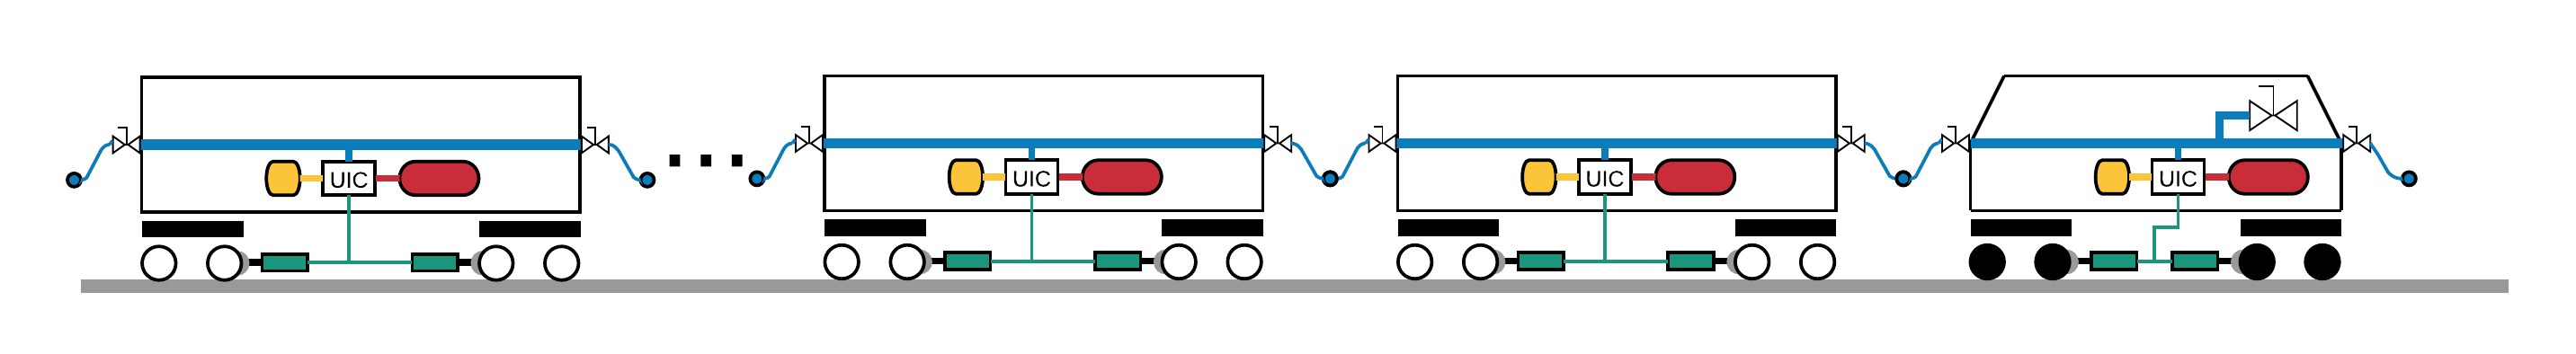
\includegraphics[width = 0.9\textwidth]{TrainBPDiagram}
\caption{Train with pneumatic automatic brake}
\label{Fig:TrainBP}
\end{center}
\end{figure*}

The braking system of a train for freely configurable train consists is designed as a distributed system, with the command line also supply pneumatic energy to the brakes along the train. These typically consist of one distributor valve per carriage or wagon and up to 12 brake actors, i.e. brake cylinders and calipers. Figure \ref{Fig:TrainBP} depicts a train setup with brake components.

The braking system of the carriages or wagons is checked qualitatively at least once every 24 h, however efficiency may vary considerably over the maintenance interval. Further, plenty of instantaneous error modes may inhibit the proper generation of a braking force by one or more actuators. This makes it necessary to consider the variation of braking distance due to these effects in the train protection system, which is achieved and communicated by help of braking curves. 

The randomised and systematic dispersion of braking performance needs to be handled according to the infrastructure composition, e.g. for infrastructure and operations providing long headways of the reliability of the braking distance prediction is not required to be as high as for dense traffic and little headway.

For a limited number of train formations, such as multiple units, the braking curve is derived from white box modelling of the braking system. Dominating parameters to be considered are:
\begin{itemize}
	\item Brake pipe: propagation velocity, flow resistances, train length
	\item Distributor valve: Filling time, brake cylinder pressure
	\item Braking force generation: efficiency, brake radius, pad/block friction coefficient
	\item Wheel/rail contact: rail surface, contaminants, slip
 	\item Discrete failure modes \cite{tsilocpas}
\end{itemize} 
The braking curve is obtained by running Monte Carlo simulations of the unit and the limited number of multiple traction formation it may operate in.

Since the amount of headway determines the utilisation of the infrastructure, it is desirable to operate trains with as short distances as possible. This may be achieved on the one hand by more reliable predictions of the braking distance and on the other hand by a shift from the current block system as depicted in Figure \ref{fig:AbsSpacDist} towards a moving block system as in Figure \ref{fig:RelBakDist}.

At this stage of operation the safety is under joint responsibility of railway undertaking and infrastructure manager, thus the confidence level required by the infrastructure is communicated to the rolling stock (ETCS onboard unit) as well as a weighting factor to increase the predicted braking distances in case of wet rails. The ETCS onboard unit is then able to use the appropriate braking curve \cite{ERAbrakingcurves}.

\subsection{Current treatment of trains}
As in the fixed block system the variation of braking performance did not play as significant a role as in the moving block system, for legacy rolling stock only the nominal braking performance was evaluated during commissioning. The nominal braking performance for freely configurable trains is typically recorded in terms of the braked weight percentage $\lambda$ \cite{uic544-1} while for multiple units and especially high speed trains, a series of retardation values along the braking curve is recorded and used to predict the braking curve.

Due to this treatment of trains, the class of freely configurable rolling stock is termed $\lambda$-braked, whereas the class of multiple units for which retardation values are recorded is termed $\gamma$-braked. As opposed to the $\gamma$-value, $\lambda$ has no direct physical meaning but offers a high degree of usability, as the braking performance of a train can be easily calculated by summation of the braked weights of the individual wagons or coaches.

With Figure \ref{Fig:BrakingCurves} in view, it is more obvious how to calculate a braking curve originating from retardation values over a velocity interval. Further it is not feasible to use the same Monte Carlo approach as for multiple units, since the amount of permissible train configurations from a set of wagons for most railway undertakings in far too high to be calculated in advance.

The European Railway Agency has conceived an approach that based its prediction on the braked weight percentages of the train, based on tests with with a large variety of trains \cite{ERAbrakingcurves}. It may be expected that the trains employed for testing are selected to be representative of the maintenance and technical of freight wagons. For this reason, trains made up of uniform wagon type which are well maintained and of current design may be treated disadvantageously. Further, the feasible amount of train testing is obviously limited compared to the confidence levels typically required by train protection systems which are in the range $\alpha = 10^{-6} \ldots 10^{-9}$.

\section{Big Data and Big Data Streams (Ingo)}
\subsection{Introduction}
In the present research on usage of Big Data in the railway system, mostly two areas are considered to gain advantage from Big Data Usage, which is on the one hand condition based maintenance, e.g. \cite{fumeo2015condition, thaduri2015railway}. The potential for savings by optimising maintenance is high in the railway business, as the lifecycle of vehicles is long and thus the maintenance cost is typically higher than the initial investment.

On the other hand, prediction of operational status as well as optimisation of railway operation, as in e.g. \cite{papa2016delay, oneto2016delay}, are fields were the data integration may be put to service profitably.

This paper deals with the interface between these two: The results of the analysis of variations in braking performance are employed to optimise operational performance of railways, however on a single wagon level which is less abstract than in pure operational approaches. At the same time, the recorded retardation data  provides insight into the maintenance state of the individual wagon, but without looking into single components.

\begin{table}  
	\begin{center}  
	\caption{Number of operated trains by DB Cargo in Germany in 2016}
	\label{Tab:Zugfahrten}
	\begin{tabular}{|c|c|}
		\hline
		\textbf{Month}	& \textbf{Freight trains operated} \\ \hline
		February & 2,641,295 \\ \hline
		March & 2,712,662 \\ \hline
		April & 2,734,730 \\ \hline
		May & 2,497,157 \\ \hline
		June & 2,719,753 \\ \hline
		July & 2,576,785 \\ \hline
		August & 2,472,119 \\ \hline
		September & 2,660,830 \\ \hline
		October & 2,513,284 \\ \hline
		November & 2,641,139 \\ \hline 
	\end{tabular}
	\end{center}
\end{table}

A common definition of Big Data is based on the 5 V \cite{hilbert2016big}:
\begin{description}
	\item[Volume:] quantity of stored and generated data 
	\item[Variety:] type and nature of the data
	\item[Velocity:] speed at which the data is generated
	\item[Variability:] potential inconsistency of the data
	\item[Veracity:] quality of the captured data
\end{description}
While neither volume nor velocity is defined concisely in order to qualify a data set as Big Data, a combination of these five criteria is likely to make Big Data approaches viable for the data set under consideration.

For the example application presented in this paper, the DB Cargo open data set \cite{DBOpenDataZug} is analysed for the number of freight trains operated (cf. Table \ref{Tab:Zugfahrten}). DB Cargo operates on average 2.6 million freight trains per month. Assume ten braking processes per train made up of 20 wagons and the braking deceleration sampled at 10 Hz during the typical braking time of approximately 90 s. At 20 bytes per sample, this yields 9.4 TB of data per month. Since freight trains operated mostly at night, assume 360 operational hours per month to calculate the peak data rate of 7.2 MB/s. While this data rate is not huge compared to other applications, its real time processing will enable to react quickly within the ETCS framework on any deterioration of braking performance.

The quantity of data for DB Cargo alone will amount to approximately 100 TB per year, which can be extrapolated by DB market share of 62 \% to approximately 150 TB per year for all freight railway undertakings in Germany. Since one peculiarity of the freight rail system is that some wagons run very frequently while others are rarely operated, this dataset needs to be kept accessible and shared between the operators in order to obtain  information on past performance of a wagon.

\subsection{MapReduce algorithm (Raphael, Ingo)}
Since current servers are not able to handle data sets of this size and streams of this velocity in an undistributed fashion, a special type of algorithm is required. One common algorithm type for Big Data applications is the MapReduce algorithm, which were introduced by Google \cite{dean2008mapreduce}.

MapReduce type algorithms use three steps for computation:
\begin{enumerate}
	\item Map: The \texttt{map()} function is applied to the local input data at each worker node. Redundant input data is ignored.
	\item Shuffle: The worker nodes redistribute the data based on output keys such that all data belonging to one output key is located on one node.
	\item Reduce: Each group of output data is processed in parallel per key. 
\end{enumerate}

The key advantage of the MapReduce scheme for Big Data is its scalability. Due to the split operation on the data in the Map and Reduce steps, it is designed for handling the dataset in multiple nodes. This removes any limitations in e.g. RAM size of the individual nodes.

\section{Proposed approach to braking performance monitoring (Raphael, Ingo)}
\subsection{Introduction}
Following the above arguments, a precise prediction of braking distances is highly desirable for performance reasons. In most countries of the world, freight rail rolling stock is comparably little advanced in terms of monitoring and connectivity. The typical freight wagon does not have power supply nor sensors. The sensible step to equip freight wagons with sensing, processing and connecting capabilities was proposed under the term \textit{Wagon 4.0} in \cite{pfaff2017stephenson}. The Wagon 4.0 makes sensing and data collection economically viable. Further it is open for further developments due to the introduction of an operating system, making the functionality described in the sequel work like a mobile phone app.

In order to keep hardware invest low and onboard technology simple, only accelerometer data is assumed to be known to the algorithm. Each wagon can be identified uniquely thanks to its wagon number. The wagons in a train can, besides some longitudinal dynamic effects, only experience the same deceleration despite different braking performance.

In this early study, no dynamic effects of e.g. brake pipe and distributor valve is taken into account, also no velocity dependent brake decelerations are recorded. Instead, only one deceleration is recorded per wagon per braking process.

\subsection{Proposed algorithm}
The algorithm to estimate the standard deviation of the braking performance is assumed to receive as an input the braking deceleration of the individual wagon. This could be achieved by e.g. using Kalman Filtering of the sensor data, possibly improved by information on the wagon weight to improve the dynamic model.

The wagon fleet data is managed in key-value-pairs $<k, v>$, the key $k$ being the unique wagon identification number and the value vector $v = \left(\sigma, n\right)$ stores the estimated standard deviation of the braking performance $\sigma$ and the number of observed braking processes $n$ for the wagon under consideration.

This deceleration due to the formation of trains is prone to be the same for all wagons in a train, thus it is difficult to estimate the variation of braking performance since the train is in fact a physical implementation of the Central Limit Theorem. 

To circumvent the convergence of the resulting distribution towards an attractor distribution, after the braking process is terminated and the observed braking deceleration is communicated to the streaming data platform, for each wagon with key $k$ a Monte-Carlo-Simulation with braking decelerations of all wagons $k_{i} \neq k$ drawn from their past observed distributions (normal distribution with standard deviation from the data store) is performed. In this way, the likely contribution of the wagon $k$ can be obtained by comparing the observed train deceleration with the results from the Monte-Carlo-Simulation.

This likely distribution of braking performance that meets the observed braking performance of the trainset is then analysed for its variance $\hat{\sigma}^2$ for each wagon $k$. This is incorporated into the prior variance $\bar{\sigma}^2$ by way of Bayesian updating, using the update \cite{gelman2014bayesian}
\begin{equation}
\sigma^2 = \frac{\hat{\sigma}^2 \bar{\sigma}^2}{\hat{\sigma}^2 + \bar{\sigma}^2}
\end{equation}

This updated standard deviation is then stored on the key value store until the next braking data arrives.

In terms of a MapReduce implementation of the proposed algorithm, this can be achieved in the following fashion:
\begin{enumerate}
	\item Map: 
	\begin{itemize}
		\item Incoming data is mapped to the individual train, using data from a second key value data storage $<k, t>$, where $k$ is the unique wagon ID and $t$ is the number of the train the wagon currently operates in.
		\item The train number $t$ serves as an output key, allowing to group all data corresponding to one train.
		\end{itemize}
	\item Shuffle: The worker nodes redistribute the data based on output keys such that all data belonging to one output key is located on one node.
	\item Reduce: 
	\begin{itemize}
		\item For each $<k, v>$, the Monte-Carlo-Simulation of the remaining wagons is performed, only requiring data present on the node.
		\item For each $<k, v>$, the Bayesian update is performed and the key value storage is updated accordingly.
		\end{itemize}
\end{enumerate}
The first operation in Reduce can be optimised by simulating all wagons $k$ only once, followed by an intermediary reduce operation to calculate the braking performance of wagon $k$.

\subsection{Numerical example}
The algorithm as described above has been executed with a small data set of $N = 100$ wagons and comparably short trains of $n = 10$ wagons each. Out of this wagon pool, $M = 100$ trains are assembled randomly and operated, with $m = 10$ braking processes observed from each train. The $<k,v>$ data storage is initialised with the conservative prior of $v = \left(2 \sigma, 0\right)$, yielding a less reliable braking distance.

Each wagon has a mass and a braking force $F_{b}$ resulting from the brake block friction coefficient, the brake rigging efficiency and the nominal brake force. The resulting brake force of each wagon is simulated to be varying following a normal distribution having a standard deviation which is itself uniformly drawn from the interval $\left[0, \sigma_{max}\right]$, where $\sigma_{max} = 0.05 F_{b}$.

The resulting braking distance is calculated for each of the operated trains, then the observed deceleration $\hat{a}$ is calculated and additive white noise having a standard deviation $\sigma_{a} = 0.05 \hat{a}$ is added. 

\begin{figure}
\begin{center}
\begin{tikzpicture}
\begin{axis}[
	name=main plot,
	%xlabel=Wagon number,
	ylabel=$\sigma$,
	xmin = 0, ymin = 0, ymax = 0.06, xmax = 100, height = 5cm, width = 8cm,
	legend entries={$\sigma$,$\hat{\sigma}$}
	]
\addplot[thick, black] table[x=No, y=SDtrue, mark = none] {TrainSim.dat};
\addplot[thick, blue, mark = none, dashed] table[x=No, y=SDest] {TrainSim.dat};
\end{axis}
\begin{axis}[
	 at={(main plot.below south west)},yshift=-3cm,
	xlabel=Wagon number,
	ylabel=$n_{\text{brakings}}$,
	xmin = 0, ymin = 0, ymax = 220, xmax = 100, height = 4cm, width = 8cm,
	]
\addplot[thick, black] table[x=No, y=n] {TrainSim.dat};
\end{axis}
\end{tikzpicture}
\caption{Comparison of estimated and true standard deviations $\hat{\sigma}$  and $\sigma$ (above), number of observed braking processes (below.)}
\label{Fig:BrakingSD}
\end{center}
\end{figure}

The MapReduce algorithm as described above is executed after each braking process, with 1000 Monte-Carlo-instances of the braking force in the Reduce stage. The results are plotted in Figure \ref{Fig:BrakingSD}, showing the good convergence of the estimated standard deviations $\hat{\sigma}$ towards the true standard deviation $\sigma$ despite the conservative prior.

\section{Conclusion and further work}
The problem of stochastic behaviour of braking performances of railway rolling stock was reviewed and put into the context of train protection systems as well as performance. The amount of data to be expected in such applications exclusively for monitoring of the braking system is determined, with the amount for this application being within a feasible dimension, however requiring appropriate data structures and algorithms.

An algorithm for the estimation of individual wagons braking performance variance from observed deceleration was proposed and formulated in the MapReduce framework, making possible to scale the software for real world applications. A numerical study shows that the algorithm converges towards the true values for a conservative prior.

The algorithm as well as the numerical study did not consider the expected value of the braking performance to be varying over time, however especially considering the typical 6 to 8 year maintenance interval and the operational conditions, such variations over time do occur and provide additional insight into the maintenance condition of the rolling stock, therefore an inclusion in future development steps appears desirable.

Further the estimation of a standard deviation may be too error prone given the typical confidence levels of train control systems of $\alpha = 10^{-6} \ldots 10^{-9}$. Therefore, a direct estimation of braking distance at a given confidence will greatly improve the applicability of the algorithm. This will require the current crude Monte-Carlo-Simulation to be replaced by an appropriate Rare Event Simulation technique, possibly also integrating discrete failure modes.

The exploitation of the time behaviour of the brake pipe system also has the potential to improve the procedure, as in this way it is more easy to identify the wagons contribution. Finally, trials using real world data will also be required to verify the procedure.


% Bibliography
% ---------------------------------------------------------------------------------
\bibliographystyle{apacite}
\bibliography{../bib}
% ---------------------------------------------------------------------------------



\section*{Biographies}

% Example bio with picture

\noindent\textbf{Raphael Pfaff} was born in Hagen, Germany in 1977. He pursued studies in Mechatronics (FH Bochum, Germany, Dipl.-Ing. (FH) 2006), Mathematics (FeU Hagen, BSc 2007) and Control Engineering (Coventry University, UK, MSc 2006, PhD 2013). He worked with Siemens and Faiveley Transport as System Engineer and Engineering Manager before receiving the call for his current position as Professor of Rail Vehicle Engineering at FH Aachen. His research interests include digitisation of railway rolling stock, reliability engineering and big data usage as well as wheel-rail contact modelling. He is scientific advisor to the Interdisciplinary Railway Research Network (IfV Bahntechnik) as well as  member of German Mathematical Society (DMV) and German Rail Engineering Society (DMG).




%\section*{Appendix}
%
%If the paper has an appendix, the appendix should appear at the end of the paper after the biographies. The appendix section is optional. 


\end{document}

